\chapterquote{'Think simple' as my old master used to say — meaning reduce the whole of its parts into the simplest terms, getting back to first principles.}{Frank Lloyd Wright}

You can angle chase to show points are collinear or lines are concurrent, lines are parallel, a line is tangent to a circle, or four points are cyclic. In computational contests, you may be asked to find an angle for easier problems and angle chasing can reveal more about the configuration for harder problems.

\section{Collinearity and Concurrency}

\begin{fact}[Collinearity Condition]
A line has measure $180^{\circ}.$ This means $A,B,C,$ are collinear if and only if for any point $P,$ $\angle ABP+\angle PBC=180^{\circ}.$ This is one of the main ways to prove points are collinear.
\end{fact}

\begin{center}
    \begin{asy}
    size(3.5cm);
    dot((0,0));
    dot((-1,0));
    dot((1,0));
    dot((-0.3,0.6));
    draw(arc((0,0),0.2,0,180));
    draw((-1,0)--(1,0));
    draw((0,0)--(-0.3,0.6));
    
    label("$A$",(-1,0),S);
    label("$B$",(0,0),S);
    label("$C$",(1,0),S);
    label("$P$",(-0.3,0.6),NW); 
    \end{asy}
\end{center}

This holds for more than one point too. For the right configuration, $A,B,C$ are collinear if and only if for points $P_1,P_2,\ldots,P_n,$ $\angle ABP_1+\angle P_1BP_2+\cdots+\angle P_nBC=180^{\circ}.$ (Directed angles can be used to avoid configuration issues.)

\begin{center}
    \begin{asy}
    size(3.5cm);
    dot((0,0));
    dot((-1,0));
    dot((1,0));
    dot((-0.3,0.6));
    dot((0.2,0.4));
    draw(arc((0,0),0.2,0,180));
    draw((-1,0)--(1,0));
    draw((0,0)--(-0.3,0.6));
    draw((0,0)--(0.2,0.4));
    
    label("$A$",(-1,0),S);
    label("$B$",(0,0),S);
    label("$C$",(1,0),S);
    label("$P_1$",(-0.3,0.6),NW);
    label("$P_2$",(0.2,0.4),NE);
    \end{asy}
\end{center}

A similar condition is that $A,B,C$ are collinear if and only if for any point $P,$ $\angle PAB=\angle PAC.$

\begin{center}
    \begin{asy}
    size(3.5cm);
    dot((0,0));
    dot((-1,0));
    dot((1,0));
    dot((-1.3,0.6));
    draw(arc((-1,0),0.2,0,120));
    draw((-1,0)--(1,0));
    draw((-1,0)--(-1.3,0.6));
    
    label("$A$",(-1,0),S);
    label("$B$",(0,0),S);
    label("$C$",(1,0),S);
    label("$P$",(-1.3,0.6),NW); 
    \end{asy}
\end{center}

\section{Parallel Lines}

\begin{fact}[Parallel Lines]
Consider parallel lines $AB$ and $CD.$ Then for $X$ on segment $AB$ and $Y$ on segment $CD,$
\[\angle AXY=180^{\circ}-\angle CYX=\angle DYX.\]
\end{fact}

\begin{center}
    \begin{asy}
    size(4cm);
    dot((-1,2));
    dot((3,6));
    dot((-5,-2));
    
    dot((1,-2));
    dot((5,2));
    dot((-3,-6));
    
    draw((-5,-2)--(3,6));
    draw((5,2)--(-3,-6));
    draw((1,-2)--(-1,2));
    
    draw(arc((1,-2),1,45,180-180atan(2)/pi));
    draw(arc((1,-2),0.9,180-180atan(2)/pi,225));
    draw(arc((-1,2),1,-135,180atan(0.5)/pi-90));
    draw((1+1.1cos((5pi/4-atan(2))/2),-2+1.1sin((5pi/4-atan(2))/2))--(1+0.9cos((5pi/4-atan(2))/2),-2+0.9sin((5pi/4-atan(2))/2)));
    draw((-1+1.1cos((-5pi/4+atan(0.5))/2),2+1.1sin((-5pi/4+atan(0.5))/2))--(-1+0.9cos((-5pi/4+atan(0.5))/2),2+0.9sin((-5pi/4+atan(0.5))/2)));
    
    label("$X$",(-1,2),NW);
    label("$A$",(-5,-2),NW);
    label("$B$",(3,6),NW);
    label("$Y$",(1,-2),SE);
    label("$D$",(5,2),SE);
    label("$C$",(-3,-6),SE);
    \end{asy}
\end{center}

\section{Angle Chasing in Circles}
We begin with some definitions.

\begin{defi}[Chord]
A chord is a line segment formed by two distinct points on a circle.
\end{defi}

\begin{defi}[Secant]
A secant is a line that intersects a circle twice.
\end{defi}

\begin{defi}[Tangent]
A tangent is a line that intersects a circle once.

Sometimes, it will be more convenient to think of a tangent as intersecting a circle twice at the same point, such as with Power of a Point.
\end{defi}

\begin{defi}[Measure of an Arc]
The measure of $\overarc{AB}$ of circle with center $O$ is the measure of $\angle AOB.$ Unless specified, this means the minor arc, or the smaller arc.
\end{defi}

Now we present three important theorems.

\begin{theo}[Inscribed Angle]
Let $A,B$ be points on a circle with center $O.$

If $C$ is a point on minor arc $AB,$ then $\angle ACB=\frac{\angle AOB}{2}.$

If $C$ is a point on major arc $AB,$ then $\angle ACB=180^{\circ}-\frac{\angle AOB}{2}.$
\end{theo}

\begin{pro}
Let $D$ be the antipode of $C.$ Then $\angle ACD=\frac{180^{\circ}-\angle AOC}{2}=\frac{\angle AOD}{2}.$ Thus addition or subtraction, depending on whether $O$ is inside acute angle $\angle ACB,$ of $\angle ACD$ and $\angle BCD$ will yield the result.
\begin{center}
    \begin{asy}
    size(4cm);
    draw(circle((0,0), 1)); 
draw((-sqrt(2)/2,-sqrt(2)/2)--(0,1)); 
draw((-sqrt(2)/2,-sqrt(2)/2)--(0,0)); 
draw((0,1)--(0,-1)); 
draw((0,1)--((sqrt(6)+sqrt(2))/4,(-sqrt(6)+sqrt(2))/4)); 
draw((0,0)--((sqrt(6)+sqrt(2))/4,(-sqrt(6)+sqrt(2))/4));

draw(arc((0,0),0.2,225,270));
draw(arc((0,1),0.2,247.5,270));

dot((0,0)); 
label("$O$", (0,0), NE); 
dot((-sqrt(2)/2,-sqrt(2)/2)); 
label("$A$", (-sqrt(2)/2,-sqrt(2)/2), SW); 
dot(((sqrt(6)+sqrt(2))/4,(-sqrt(6)+sqrt(2))/4));
label("$B$", ((sqrt(6)+sqrt(2))/4,(-sqrt(6)+sqrt(2))/4), SE); 
dot((0,1)); 
label("$C$", (0,1), N); 
dot((0,-1)); 
label("$D$", (0,-1), S);
    \end{asy}
\end{center}
\end{pro}

\begin{theo}[Tangent Perpendicular to Radius]
Consider circle $\omega$ with center $O$ and point $P$ on $\omega.$ If $\ell$ is the tangent to $\omega$ through $P,$ then $\ell$ is perpendicular to $OP.$
\end{theo}

\begin{pro}
This is identical to the claim that $P$ is the point on $\ell$ with the smallest distance to $O.$ We prove this is true by contradiction. Assume this is not true. Then there is some point $X$ on $\ell$ such that $OX<OP,$ implying that $\ell$ intersects $\omega$ twice, contradiction. 
\begin{center}
    \begin{asy}
    size(4cm);
    draw(circle((0,0), 1));
    dot((0,-1));
    dot((0,0));
    draw((-2,-1)--(2,-1));
    draw((0,-1)--(0,0));
    
    label("$P$",(0,-1),S);
    label("$O$",(0,0),N);
    \end{asy}
\end{center}
\end{pro}

\begin{theo}[Tangent Angle]
Consider circle $\omega$ with center $O$ and points $A,B$ on $\omega.$ Let $\ell$ be the tangent to $\omega$ through $B$ and let $\theta$ be the acute angle between $AB$ and $\ell.$ Then $\theta=\frac{\angle AOB}{2}.$
\end{theo}

\begin{pro}
Let $B'$ be the antipode of $B.$ Then note that $\theta=90^{\circ}-\angle ABB'=\frac{180^{\circ}-\angle AOB'}{2}=\frac{\angle AOB}{2}.$
\begin{center}
    \begin{asy}
    size(4cm);
    draw(circle((0,0), 1));
    dot((0,-1));
    dot((0.8,-0.6));
    dot((0,1));
    draw((0.8,-0.6)--(0,-1));
    draw((-2,-1)--(2,-1));
    draw((0,-1)--(0,1));
    
    label("$B$",(0,-1),S);
    label("$B'$",(0,1),N);
    label("$A$",(0.8,-0.6),NW);
    \end{asy}
\end{center}
\end{pro}

A corollary of this theorem is that if $C$ is some point on $\overarc{AB},$ then $\theta=\angle ACB.$

With the Inscribed Angle Theorem in mind, try to prove these two theorems.

\begin{theo}[Angle of Secants/Tangents]
Let lines $AX$ and $BY$ intersect at $P$ such that $A,X,P$ and $B,Y,P$ are collinear in that order. Then $\angle APB=\frac{\angle AOB-\angle XOY}{2}.$

\begin{center}
    \begin{asy}
    size(4cm);
    draw(circle((0,0), 1)); 
draw((-1.5137699061468413,-0.5200439036267299)--(0.5006080051165431,0.8656740871790233)); 
draw((-1.5137699061468413,-0.5200439036267299)--(0.8698306996792652,-0.49335033586233623)); 

dot((-1.5137699061468413,-0.5200439036267299)); 
label("$P$", (-1.5137699061468413,-0.5200439036267299), NW); 
dot((0.5006080051165431,0.8656740871790233)); 
label("$A$", (0.5006080051165431,0.8656740871790233), NE); 
dot((0.8698306996792652,-0.49335033586233623)); 
label("$B$", (0.8698306996792652,-0.49335033586233623), NW); 
dot((-0.98744289059587,-0.15797638371501177)); 
label("$X$", (-0.98744289059587,-0.15797638371501177), NW); 
dot((-0.858564029240042,-0.5127063562070442)); 
label("$Y$", (-0.858564029240042,-0.5127063562070442), NE); 
    \end{asy}
\end{center}

\begin{hint}
\begin{addhint}
{How can you express $\frac{\angle DOE}{2}$ and $\frac{\angle AOB}{2}?$}
\end{addhint}
\begin{addhint}
{Draw $AE.$}
\end{addhint}
\begin{addhint}
{Look at $\angle AEC.$}
\end{addhint}
\end{hint}
\end{theo}

\begin{theo}[Angle of Chords]
Let chords $AC,BD$ intersect at $P.$ Then $\angle APB=\frac{\angle AOB+\angle COD}{2}.$
\begin{center}
    \begin{asy}
    size(3.5cm);
    draw(arc((-0.002944953385821347,0.1945321088804997),0.25,396.63059336924744,499.02864317828227)); 

draw(circle((0,0), 1)); 
draw((-0.6520239138456277,0.758198401326084)--(0.8421035046648182,-0.5393159439801781)); 
draw((0.6982426762645825,0.7158611353068928)--(-0.8866287744814202,-0.462481801005807)); 

dot((-0.6520239138456277,0.758198401326084)); 
label("$A$", (-0.6520239138456277,0.758198401326084), NW); 
dot((0.6982426762645825,0.7158611353068928)); 
label("$B$", (0.6982426762645825,0.7158611353068928), NE); 
dot((0.8421035046648182,-0.5393159439801781)); 
label("$C$", (0.8421035046648182,-0.5393159439801781), SE); 
dot((-0.8866287744814202,-0.462481801005807)); 
label("$D$", (-0.8866287744814202,-0.462481801005807), SW); 
dot((-0.002944953385821347,0.1945321088804997)); 
label("$P$", (-0.002944953385821347,0.1945321088804997), S); 
\end{asy}
\end{center}

\begin{hint}
\begin{addhint}
{Note $\angle APB=180^{\circ}-\angle BAP-\angle ABP.$}
\end{addhint}
\end{hint}
\end{theo}

\section{Cyclic Quadrilaterals}

Here's a very important application of the Inscribed Angle Theorem.

\begin{theo}[Cyclic Quadrilaterals]
Any one of the three implies the other two:
\begin{enumerate}
    \item Quadrilateral $ABCD$ is cyclic.
    
    \item $\angle ABC+\angle ADC=180^{\circ}.$
    
    \item $\angle BAC=\angle BDC.$
\end{enumerate}
\begin{center}
\begin{asy}
size(3.5cm);

draw(circle((0,0), 1)); 

dot((-0.6520239138456277,0.758198401326084)); 
label("$A$", (-0.6520239138456277,0.758198401326084), NW); 
dot((0.6982426762645825,0.7158611353068928)); 
label("$B$", (0.6982426762645825,0.7158611353068928), NE); 
dot((0.8421035046648182,-0.5393159439801781)); 
label("$C$", (0.8421035046648182,-0.5393159439801781), SE); 
dot((-0.8866287744814202,-0.462481801005807)); 
label("$D$", (-0.8866287744814202,-0.462481801005807), SW); 

draw((-0.6520239138456277,0.758198401326084)--(0.6982426762645825,0.7158611353068928)--(0.8421035046648182,-0.5393159439801781)--(-0.8866287744814202,-0.462481801005807)--cycle);
\end{asy}
\begin{asy}
size(3.5cm);
draw(arc((-0.6520239138456277,0.758198401326084),0.3352236296243588,319.02864317828227,358.2040937604978)); 
draw(arc((-0.8866287744814202,-0.462481801005807),0.3352236296243588,357.45514278703183,396.63059336924744)); 

draw(circle((0,0), 1)); 
draw((0.6982426762645825,0.7158611353068928)--(-0.6520239138456277,0.758198401326084)); 
draw((-0.6520239138456277,0.758198401326084)--(0.8421035046648182,-0.5393159439801781)); 
draw((0.6982426762645825,0.7158611353068928)--(-0.8866287744814202,-0.462481801005807)); 
draw((-0.8866287744814202,-0.462481801005807)--(0.8421035046648182,-0.5393159439801781)); 
draw(arc((-0.6520239138456277,0.758198401326084),0.3352236296243588,319.02864317828227,358.2040937604978)); 
draw((-0.3762942045336219,0.650231969055075)--(-0.3034599416964878,0.6217125341155632)); 
draw(arc((-0.8866287744814202,-0.462481801005807),0.3352236296243588,357.45514278703183,396.63059336924744)); 
draw((-0.6035182048501434,-0.37569454123994417)--(-0.5287342807965981,-0.35276960469801844));

dot((-0.6520239138456277,0.758198401326084)); 
label("$A$", (-0.6520239138456277,0.758198401326084), NW); 
dot((0.6982426762645825,0.7158611353068928)); 
label("$B$", (0.6982426762645825,0.7158611353068928), NE); 
dot((0.8421035046648182,-0.5393159439801781)); 
label("$C$", (0.8421035046648182,-0.5393159439801781), SE); 
dot((-0.8866287744814202,-0.462481801005807)); 
label("$D$", (-0.8866287744814202,-0.462481801005807), SW);
\end{asy}
\end{center}
\end{theo}

\section{Examples}
We present several examples of angle chasing problems, sorted by ``flavor.''

\subsection{Computational Problems}
This is a compilation of computational problems meant to serve as low-level examples for first-time readers. If this is your first time encountering the material, I strongly suggest you focus on this section.
\begin{exam}[AMC 10B 2011/18]
Rectangle $ABCD$ has $AB = 6$ and $BC = 3$. Point $M$ is chosen on side $AB$ so that $\angle AMD = \angle CMD$. What is the degree measure of $\angle AMD?$
\end{exam}

\begin{sol}
Note that $\angle CMD=\angle AMD=\angle AMD=\angle MDC,$ implying that $CM=CD=6.$ Thus $\angle BMC=30^{\circ},$ implying that $\angle AMD=75^{\circ}.$
\begin{center}
\begin{asy}
size(4cm);

pair A=(0,3), B=(6,3), C=(6,0), D=(0,0);
pair M=(0.80385,3);

draw(A--B--C--D--cycle);
draw(M--C);
draw(M--D);

dot("$A$",A,NW);
dot("$B$",B,NE);
dot("$C$",C,SE);
dot("$D$",D,SW);
dot("$M$",M,N);
\end{asy}
\end{center}
\end{sol}

\begin{exam}
Two circles $\omega_1,\omega_2$ intersect at $P,Q.$ If a line intersects $\omega_1$ at $A,B$ and $\omega_2$ at $C,D$ such that $A,B,C,D$ lie on the lie in that order, and $P$ and $Q$ lie on the same side of the line, compute the value of $\angle APC+\angle BQD.$
\end{exam}

\begin{sol}
Without loss of generality, let $P$ be closer to $\ell$ than $Q.$ Note
\[\angle APC=180-\angle PAB-\angle BCP=\angle DCP-\angle PAB\]\[\angle BQD=\angle BQP+\angle DQP.\]Since $\angle PAB=\angle BDP,$ the sum is $\angle DCP+\angle DQP=180.$
\end{sol}

\subsection{Construct the Diagram}
These problems are very simple; just construct the diagram and the problem will solve itself for you.

\begin{exam}[USA EGMO TST 2020/4]
Let $ABC$ be a triangle. Distinct points $D$, $E$, $F$ lie on sides $BC$, $AC$, and $AB$, respectively, such that quadrilaterals $ABDE$ and $ACDF$ are cyclic. Line $AD$ meets the circumcircle of $\triangle ABC$ again at $P$. Let $Q$ denote the reflection of $P$ across $BC$. Show that $Q$ lies on the circumcircle of $\triangle AEF$.
\end{exam}

\begin{sol}
Note that $Q$ is the intersection of $BE$ and $CF,$ since $\angle EBD=\angle CAP=\angle CBP$ and $\angle FCB=\angle BAO=\angle BCP.$ Now note that $\angle BQC=\angle BPC=180^{\circ}-\angle A.$

\begin{center}
\begin{asy}
size(6cm);
//import geometry;

point A=(0.5,3);
point B=(0,0);
point C=(4,0);
point D=(B+C)/2.5;

circle O1=circle(A,B,D);
circle O2=circle(A,C,D);
circle cABC=circle(A,B,C);

point E_=intersectionpoints(O1, line(A,C))[0];
point F=intersectionpoints(O2, line(A,B))[0];
point P=intersectionpoints(cABC, line(A,D))[0];
point Q=reflect(B,C)*P ;
point M=(P+Q)/2 ;

draw(A--B--C-- cycle );
draw(O1 ^^ O2 ^^ cABC);
draw(B--Q--C,blue);
draw(B--P--C);
draw(F--Q--E_, blue);
//draw(A--P ^^ P--Q , gray);

dot("$A$", A, N+W);
dot("$B$", B, S+W);
dot("$C$", C, E+S);
dot("$D$", D, 2*S+W);
dot("$E$", E_, E+N);
dot("$F$", F, W);
dot("$P$", P, S);
dot("$Q$", Q, N);
\end{asy}
\end{center}
\end{sol}

\subsection{Tangent Angle Criterion}
When tangent lines are given, you have to pay close attention the the tangent angle criterion.

\begin{exam}[British Math Olympiad Round 1 2000/1]
Two intersecting circles $C_1$ and $C_2$ have a common tangent which touches $C_1$ at $P$ and $C_2$ at $Q.$ The two circles intersect at $M$ and $N,$ where $N$ is nearer to $PQ$ than $M$ is. The line $PN$ meets the circle $C_2$ again at $R.$ Prove that $MQ$ bisects angle $PMR.$
\end{exam}

\begin{sol}
Note that $\angle RMQ=180-\angle RNQ=180-(\angle PNM+\angle QNM)=180-(\angle QPM+\angle PQM)=\angle PMQ.$
\end{sol}

\subsection{Orthocenter}
Sometimes a problem will ask you to prove that $AH\perp BC$ for some point $H$ not on $BC.$ This is generally difficult to do directly, and one of the more elementary methods used is to show that $H$ is the orthocenter of $\triangle ABC,$ or $BH\perp CA$ and $CH\perp AB.$

This is obviously not always going to be true, so make sure that this actually seems true before you try too hard to prove it.

\begin{exam}[Swiss Math Olympiad 2007/4]
Let $ABC$ be an acute-angled triangle with $AB> AC$ and orthocenter $H$. Let $D$ be the projection of $A$ on $BC$. Let $E$ be the reflection of $C$ about $D$. The lines $AE$ and $BH$ intersect at point $S$. Let $N$ be the midpoint of $AE$ and let $M$ be the midpoint of $BH$. Prove that $MN$ is perpendicular to $DS$.
\end{exam}

\begin{sol}
We claim $S$ is the orthocenter of $\triangle DEM.$ To do this, it suffices to show that $SN\perp DM$ and $SM\perp DN.$ Let $H'$ be the second intersection of $AH$ with $(ABC).$

Note that $DM\parallel BH'$ by a homothety about $H,$ $\angle MAE=\angle DAC=90^{\circ}-\angle C,$ and $\angle AMB=\angle C,$ proving $SN\perp DM.$

Now note that $DN\parallel AC$ by a homothety about $E,$ proving $SM\perp DN.$
\end{sol}

\section{Summary}

\subsection{Theory}

\begin{enumerate}
    \item Supplementary Angles
    
    \begin{itemize}
    
    \Item $A,B,C,$ are collinear if and only if for any point $P,$ $\angle ABP+\angle PBC=180^{\circ}.$
    
    \Item This is generalizable to more points.
    
    \Item $A,B,C$ are collinear if and only if for any point $P,$ $\angle PAB=\angle PAC.$
    
    \end{itemize}
 
    \item Parallel Lines
    
    \begin{itemize}
    
    \Item For parallel lines $AB,CD$ and points $X$ and $Y$ on $AB$ and $CD$ respectively, $\angle AXY=180^{\circ}-\angle CXY=\angle DXY.$
    
    \end{itemize}
    
    \item Inscribed Angle Theorem
    
    \begin{itemize}
    
    \Item The measure of an angle is half the measure of the subtended arc.
    
    \Item Proved by considering the case where one leg of the angle is a diameter and angle chasing, and generalizing.
    
    \Item Thale's Theorem: In the special case where the feet of the angle form a diameter of the circle, the angle is $90^{\circ}.$ The converse also holds.
    
    \end{itemize}
    
    \item Tangent Perpendicular to Radius
    
    \begin{itemize}
    
    \Item This is important. Remember it.
    
    \end{itemize}
    
    \item Tangent Angle
    
    \begin{itemize}
    
    \Item When you see circles and an angle condition with a tangent, keep this in mind.
    
    \Item This proves points are concyclic.
    
    \end{itemize}
    
    \item Cyclic Quadrilaterals
    
    \begin{itemize}
    
    \Item Angles on opposite sides are supplementary.
    
    \Item Angles on the same side are congruent.
    
    \end{itemize}
\end{enumerate}

\subsection{Tips and Strategies}

\begin{enumerate}
    \item Proving collinearity and concurrency for lines can basically be switched around at will.
    
    \item One way to prove concurrency of three figures is to let two of them intersect at a point $P,$ and prove the third passes through $P.$
    
    \item If two lines are parallel, then it's probably an important part of the problem.
    
    \item The same is true for tangent lines.
    
    \item A nice way to show that $AH\perp BC$ is to show that $H$ is the orthocenter of $\triangle ABC,$ namely, $BH\perp CA$ and $CH\perp AB.$
    \begin{itemize}
    \Item This will not always be true - make sure that it seems true before you try too hard to prove it.
    \end{itemize}
\end{enumerate}

\pagebreak

\section{Exercises}

\subsection{Check-ins}
\begin{enumerate}
    \item Prove $\triangle ABC$ satisfies $\angle A+\angle B+\angle C=180^{\circ}.$
    \begin{hint}
    \begin{addhint}
    {Draw a line through $A$ parallel to $BC.$}
    \end{addhint}
    \end{hint}

    \item Prove that the sum of the interior angles of an $n-gon$ is $180(n-2).$
    \begin{hint}
    \begin{addhint}
    {Reduce the problem to a bunch of triangles.}
    \end{addhint}
    \begin{addhint}
    {Pick a point. Draw all the diagonals connected to that point.}
    \end{addhint}
    \end{hint}

    \item (Brazil 2004) In the figure, $ABC$ and $DAE$ are isosceles triangles ($AB = AC = AD = DE$) and the angles $BAC$ and $ADE$ have measures $36^{\circ}$.
\begin{enumerate}
    \item Using geometric properties, calculate the measure of angle $\angle EDC$.
    \item Knowing that $BC = 2$, calculate the length of segment $DC$.
    \item Calculate the length of segment $AC$.
\end{enumerate}
\begin{center}
\begin{asy}
import olympiad;
size(4cm);
pair A=(0,0),B=dir(0),C=dir(36),D=dir(72),E=(2cos(0.4pi),0);
dot(A^^B^^C^^D^^E);
draw(A--B--C--cycle);
draw(A--D--E);
draw(D--C,dotted);
label("A",A,dir(-90));
label("B",B,dir(-90));
label("C",C,dir(40));
label("D",D,dir(90));
label("E",E,dir(-90));
\end{asy}
\end{center}

    \item If $\angle ABC=60^{\circ}$ and $\angle CAB=70^{\circ},$ find $\overarc{AB}-\overarc{DE}.$
    
    \begin{center}
    \begin{asy}
    size(4cm);
    draw(circle((0,0), 1)); 
draw((-1.5137699061468413,-0.5200439036267299)--(0.5006080051165431,0.8656740871790233)); 
draw((-1.5137699061468413,-0.5200439036267299)--(0.8698306996792652,-0.49335033586233623)); 

dot((-1.5137699061468413,-0.5200439036267299)); 
label("$C$", (-1.5137699061468413,-0.5200439036267299), NW); 
dot((0.5006080051165431,0.8656740871790233)); 
label("$A$", (0.5006080051165431,0.8656740871790233), NE); 
dot((0.8698306996792652,-0.49335033586233623)); 
label("$B$", (0.8698306996792652,-0.49335033586233623), NW); 
dot((-0.98744289059587,-0.15797638371501177)); 
label("$D$", (-0.98744289059587,-0.15797638371501177), NW); 
dot((-0.858564029240042,-0.5127063562070442)); 
label("$E$", (-0.858564029240042,-0.5127063562070442), NE); 
    \end{asy}
    \end{center}
    
    \item
    
    \begin{enumerate}
        \item Given that $A, B, C,$ and $D$ are all on the same circle, that $BE$ is the angle bisector of $\angle{ABC},$ that $\angle{AEB}=\angle{CEB},$ and that $\angle{ADC}=50^{\circ},$ find $\angle{BAC}.$
    
        \item Given points $A,B,C,D,E$ such that $BE$ is the angle bisector of $\angle{ABC},$ $\angle{AEB}=\angle{CEB},$ $\angle{BAC} + \angle{BDC} = \angle{ABD} + \angle{ACD},$ and $\angle{ADC}=48^{\circ}, $ find $\angle{BCA.}$
    \end{enumerate}
  
    \item Consider any cyclic pentagon $ABCDE$. If $P$ is the center of $(ABCDE),$ then prove that $ABCP$ is never cyclic.
    
    \item Two circles $\omega_1,\omega_2$ intersect at $P,Q.$ If a line intersects $\omega_1$ at $A,B$ and $\omega_2$ at $C,D$ such that $A,B,C,D$ lie on the lie in that order, and $P$ and $Q$ lie on the same side of the line, compute $\angle APC+\angle BQD.$
	\begin{solu}
	\begin{addsol}
	{Without loss of generality, let $P$ be closer to $\ell$ than $Q.$ Note
	\[\angle APC=180-\angle PAB-\angle BCP=\angle DCP-\angle PAB\]\[\angle BQD=\angle BQP+\angle DQP.\]Since $\angle PAB=\angle BDP,$ the sum is $\angle DCP+\angle DQP=180.$}
	\end{addsol}
	\end{solu}
\end{enumerate}

\subsection{Problems}

\begin{enumerate}
    \item Consider rectangle $ABCD$ with $AB = 6,$ $BC = 8.$ Let $M$ be the midpoint of $AD$ and let $N$ be the midpoint of $CD.$ Let $BM$ and $BN$ intersect $AC$ at $X$ and $Y$ respectively. Find $XY.$

    \item (AMC 10A 2019/13) Let $\triangle ABC$ be an isosceles triangle with $BC = AC$ and $\angle ACB = 40^{\circ}$. Construct the circle with diameter $\overline{BC}$, and let $D$ and $E$ be the other intersection points of the circle with the sides $\overline{AC}$ and $\overline{AB}$, respectively. Let $F$ be the intersection of the diagonals of the quadrilateral $BCDE$. What is the degree measure of $\angle BFC?$ \begin{hint}
    \begin{addhint}
    {What is $\angle BCD?$}
    \end{addhint}
    \end{hint}
    
    \item (Miquel's Theorem) Consider $\triangle ABC$ with $D$ on $BC,$ $E$ on $CA,$ and $F$ on $AB.$ Prove that $(AEF),$ $(BFD),$ and $(CDE)$ concur. \begin{hint}
    \begin{addhint}
    {Let $(BFD)$ intersect $(CDE)$ at $P.$}
    \end{addhint}
    \end{hint}
    
    \item Consider $\triangle ABC$ with $D$ on segment $BC,$ $E$ on segment $CA,$ and $F$ on segment $AB.$ Let the circumcircles of $\triangle FBD$ and $\triangle EFA$ intersect at $P\neq D.$ If $\angle A=50^{\circ},\angle B=35^{\circ},$ find $\angle DPE.$
    
    \item Let circles $\omega_1$ and $\omega_2$ intersect at $X,Y.$ Let line $\ell_1$ passing through $X$ intersect $\omega_1$ at $A$ and $\omega_2$ at $C,$ and let line $\ell_2$ passing through $Y$ intersect $\omega_1$ at $B$ and $\omega_2$ at $D.$ If $\ell_1$ intersects $\ell_2$ at $P,$ prove that $\triangle PAB\sim \triangle PCD.$ \begin{hint}
    \begin{addhint}
    {What information do cyclic quadrilaterals give you?}
    \end{addhint}
    \end{hint}
    
    \item (Reim's Theorem) Let circles $\omega_1,\omega_2$ intersect at $P,Q.$ Let line $\ell_1$ passing through $P$ intersect $\omega_1$ again at $A_1$ and $\omega_2$ again at $A_2.$ Let $B_1$ be a point on $\omega_1$ and $B_2$ be a point on $\omega_2.$ Then prove that $A_1B_1\parallel A_2B_2$ if and only if $Q$ lies on $B_1B_2.$
    
    \item (Simson's Theorem) Consider $\triangle ABC$ and point $P,$ and let $X,Y,Z$ be the feet of the altitudes from $P$ to $BC,CA,AB.$ Prove that $X,Y,Z$ are collinear if and only if $P$ is on $(ABC).$ \begin{hint}
    \begin{addhint}
    {There are three more cyclic quadrilaterals.}
    \end{addhint}
    \end{hint}
    
    \item (AMC 10B 2011/17) In the given circle, the diameter $\overline{EB}$ is parallel to $\overline{DC}$, and $\overline{AB}$ is parallel to $\overline{ED}$. The angles $AEB$ and $ABE$ are in the ratio $4 : 5$. What is the degree measure of angle $BCD?$

\begin{center}
\begin{asy}
import olympiad;

size(4cm);

real r=3;
pair A=(-3cos(80),-3sin(80));
pair D=(3cos(80),3sin(80)), C=(-3cos(80),3sin(80));
pair O=(0,0), E=(-3,0), B=(3,0);
path outer=Circle(O,r);
draw(outer);
draw(E--B);
draw(E--A);
draw(B--A);
draw(E--D);
draw(C--D);
draw(B--C);

pair[] ps={A,B,C,D,E,O};
dot(ps);

label("$A$",A,N);
label("$B$",B,NE);
label("$C$",C,S);
label("$D$",D,S);
label("$E$",E,NW);
\end{asy}
\end{center}

\item (Formula of Unity 2018) A point $O$ is the center of an equilateral triangle $ABC.$ A circle that passes through points $A$ and $O$ intersects the sides $AB$ and $AC$ at points $M$ and $N$ respectively. Prove that $AN=BM.$
\begin{solu}
\begin{addsol}
{Note that $\angle MBO=30^{\circ}=\angle NAO,$ $\angle ANO=180^{\circ}-\angle AMO=\angle BMO,$ and $AO=BO,$ so $\triangle BMO\cong \triangle ANO.$ Thus $AN=BM.$}
\end{addsol}
\end{solu}

\item (Australia Math Olympiad 2019/3) Let $A,B,C,D,E$ be five points in order on a circle $K$. Suppose that $AB = CD$ and $BC = DE$. Let the chords $AD$ and $BE$ intersect at the point $P$. Prove that the circumcentre of triangle $AEP$ lies on $K$.
\begin{hint}
\begin{addhint}
{Equal sides mean equal arclengths.}
\end{addhint}
\begin{addhint}
{Look for parallel lines.}
\end{addhint}
\begin{addhint}
{$BCDP$ is a parallelogram.}
\end{addhint}
\end{hint}
\begin{solu}
\begin{addsol}
{The central claim is that $BCDP$ is a parallelogram. Note that $ED=CB$ implies $EB\parallel DC,$ and similarly, $AB=CD$ implies $AD\parallel BC.$

Note note $\angle AKE=180^{\circ}=2\angle APE=360^{\circ}-2\angle BPD=360^{\circ}-2\angle BCD.$ Also note that $2\angle BCD-\angle ACE=180^{\circ},$ so $\angle ACE=2\angle BCD-180^{\circ}.$

Thus $\angle AKE+\angle ACE=180^{\circ},$ as desired.}
\end{addsol}
\end{solu}

\item Consider square $ABCD$ and some point $P$ outside $ABCD$ such that $\angle APB=90^{\circ}.$ Prove that the angle bisector of $\angle APB$ also bisects the area of $ABCD.$
\begin{hint}
\begin{addhint}
{Add stuff so that the angle bisector of $\angle APB$ the diagonal of a square as well.}
\end{addhint}
\end{hint}
\begin{solu}
\begin{addsol}
{Let $Q,R,S$ be the rotations of $P$ about $O$ by $90^{\circ},180^{\circ},270^{\circ}$ counterclockwise. Note that $PR$ is the angle bisector of $\angle APB$ and $PR$ bisects the area of $[PQRS].$ Since the area we added to both halves of $ABCD$ is the same, $PR$ also bisects $ABCD.$

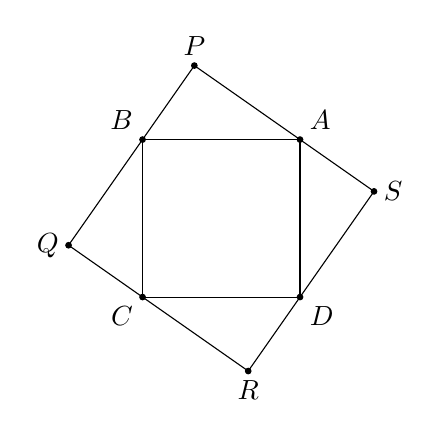
\begin{tikzpicture}
    \draw (-1,-1)--(-1,1)--(1,1)--(1,-1)--cycle;
    \filldraw (-1,-1) circle (1pt) node[anchor=north east] {$C$};
    \filldraw (-1,1) circle (1pt) node[anchor=south east] {$B$};
    \filldraw (1,1) circle (1pt) node[anchor=south west] {$A$};
    \filldraw (1,-1) circle (1pt) node[anchor=north west] {$D$};
    
    \draw (-0.342020143,1.93969262)--(1.93969262,0.342020143)--(0.342020143,-1.93969262)--(-1.93969262,-0.342020143)--cycle;
    \filldraw (-0.342020143,1.93969262) circle (1pt) node[anchor=south] {$P$};
    \filldraw (1.93969262,0.342020143) circle (1pt) node[anchor=west] {$S$};
    \filldraw (0.342020143,-1.93969262) circle (1pt) node[anchor=north] {$R$};
    \filldraw (-1.93969262,-0.342020143) circle (1pt) node[anchor=east] {$Q$};
    \end{tikzpicture}}
\end{addsol}
\end{solu}

\item (USAJMO 2020/4) Let $ABCD$ be a convex quadrilateral inscribed in a circle and satisfying $DA < AB = BC < CD$. Points $E$ and $F$ are chosen on sides $CD$ and $AB$ such that $BE \perp AC$ and $EF \parallel BC$. Prove that $FB = FD$.

\item (IMO 2006/1) Let $ABC$ be triangle with incenter $I$. A point $P$ in the interior of the triangle satisfies\[\angle PBA+\angle PCA = \angle PBC+\angle PCB.\]Show that $AP \geq AI$, and that equality holds if and only if $P=I$.

\end{enumerate}

\subsection{Challenges}

\begin{enumerate}

	\item (MAST Diagnostic 2020) Consider parallelogram $ABCD$ with $AB=7,$ $BC=6.$ Let the angle bisector of $\angle DAB$ intersect $BC$ at $X$ and $CD$ at $Y.$ Let the line through $X$ parallel to $BD$ intersect $AD$ at $Q.$ If $QY=6,$ find $\cos\angle DAB.$
	\begin{hint}
	\begin{addhint}
	{How would you find $BX$ and $DY?$}
	\end{addhint}
	\begin{addhint}
	{Remember that $QX$ and $DB$ are parallel. How does this help you find $QD?$}
	\end{addhint}
	\end{hint}
	\begin{solu}
	\begin{addsol}
	{Note that $\triangle ABX$ and $\triangle ADY$ are isosceles, so $BX=7$ and $DY=6.$ Now also note that $XQDB$ is a parallelogram, so $QD=BX=7.$ Now note $\angle QDY=\angle DAB,$ so it suffices to find $\cos\angle QDY.$
	
	Now note that $QY=DY=6$ and $QD=7.$ Thus dropping the altitude from $Y$ to $QD$ gives us $\cos \angle QDY=\frac{\frac{7}{2}}{6}=\frac{7}{12}.$}
	\end{addsol}
	\end{solu}

    \item (Memorial Day Mock AMC 10 2018/21) In the following diagram, $m\angle BAC=m\angle BFC=40^{\circ}$, $m\angle ABF=80^{\circ}$, and $m\angle FEB=2m\angle DBE=2m\angle FBE$. What is $m\angle ADB$?

    \begin{center}
    \begin{asy}
    size(4cm);
    draw((0,0)--(-14,0)--(2,8)--(0,0)--(-9,2.5)--(-5.5,0)--(-6,4)--cycle);
    draw((-5.5,0)--(2,8));
    label("A", (2,8), NE);
    label("B", (0,0), SE);
    label("C", (-5.5,0), S);
    label("D", (-14,0), SW);
    label("E", (-9,2.5), NNW);
    label("F", (-6,4), NNW);
    \end{asy}
    \end{center}
    
    \begin{hint}
    \begin{addhint}
    {Look for cyclic quadrilaterals.}
    \end{addhint}
    \begin{addhint}
    {Use Tangent/Secant to set up a system of equations.}
    \end{addhint}
    \end{hint}
    
    \item (FARML 2012/6) In triangle $ABC,$ $AB=7,$ $AC=8,$ and $BC=10.$ $D$ is on $AC$ and $E$ is on $BC$ such that $\angle AEC=\angle BED=\angle B+\angle C.$ Compute the length $AD.$
    \begin{hint}
    \begin{addhint}
    {Look for similar triangles.}
    \end{addhint}
    \begin{addhint}
    {Prove $\triangle ABC\sim \triangle EDC\sim \triangle EBA.$}
    \end{addhint}
    \end{hint}
    \begin{solu}
\begin{addsol}
{Angle chase to find $\triangle ABC\sim \triangle EDC\sim \triangle EBA.$ So $BE=7\cdot\frac{7}{10}=\frac{49}{10},$ implying $CE=10-\frac{49}{10}=\frac{51}{10},$ and $CD=\frac{10}{8}\cdot\frac{51}{10}=\frac{51}{8},$ implying $AD=8-\frac{51}{8}=\frac{13}{8}.$}
\end{addsol}
\end{solu}
    
    \item (ISL 1994/G1) $C$ and $D$ are points on a semicircle. The tangent at $C$ meets the extended diameter of the semicircle at $B$, and the tangent at $D$ meets it at $A$, so that $A$ and $B$ are on opposite sides of the center. The lines $AC$ and $BD$ meet at $E$. $F$ is the foot of the perpendicular from $E$ to $ AB$. Show that $EF$ bisects angle $CFD.$
    \begin{hint}
    \begin{addhint}
    {Where do $BC$ and $DA$ meet?}
    \end{addhint}
    \begin{addhint}
    {Draw in the center of the semicircle.}
    \end{addhint}
    \begin{addhint}
    {Look for similar triangles.}
    \end{addhint}
    \end{hint}
    \begin{solu}
    \begin{addsol}
    {The key observation is that $AD,BC,EF$ concur.
    
    Let $AD$ and $BC$ intersect at $P$ and let $Q$ be the foot of the altitude from $P$ to $AB.$ Also let the semicircle have center $O.$ Now note
    \[\triangle PAQ\sim \triangle OAD\]
    \[\triangle PBQ\sim \triangle OBC\]
    so $\frac{AQ}{QB}\cdot\frac{BC}{CP}\cdot\frac{PD}{DA}=1.$ Since $AC,BD,PQ$ concur, $Q$ is actually $F,$ and $AC,BD,PF$ concur.
    
    Now note
    \[\angle OCP=\angle ODP=\angle OFP=90^{\circ},\]
    so $OFCPD$ is cyclic. Thus
    \[\angle COP=\angle DOP\]
    \[\angle CFP=\angle DFP.\]}
    \end{addsol}
    \end{solu}
    
    \item Consider $\triangle ABC$ with $D$ on line $BC.$ Let the circumcenters of $\triangle ABD$ and $\triangle ACD$ be $M,N,$ respectively. Let the circumcircle of $\triangle MND$ intersect the circumcircle of $\triangle ACD$ again at $H\neq D.$ Prove that $A,M,H$ are collinear.
    \begin{hint}
    \begin{addhint}
    {Look for similar and congruent triangles.}
    \end{addhint}
    \begin{addhint}
    {What does $\triangle AMN\sim\triangle DMN\sim\triangle ABC$ tell you?}
    \end{addhint}
    \end{hint}
    
    \item (APMO 1999/3) Let $\Gamma_1$ and $\Gamma_2$ be two circles intersecting at $P$ and $Q$. The common tangent, closer to $P$, of $\Gamma_1$ and $\Gamma_2$ touches $\Gamma_1$ at $A$ and $\Gamma_2$ at $B$. The tangent of $\Gamma_1$ at $P$ meets $\Gamma_2$ at $C$, which is different from $P$, and the extension of $AP$ meets $BC$ at $R$.
Prove that the circumcircle of triangle $PQR$ is tangent to $BP$ and $BR$.
    \begin{hint}
    \begin{addhint}
    {Show that $BP=BR.$}
    \end{addhint}
    \begin{addhint}
    {$R$ seems somewhat pesky. Can you find other stuff $R$ is involved with?}
    \end{addhint}
    \begin{addhint}
    {Prove that $ABRQ$ is cyclic.}
    \end{addhint}
    \begin{addhint}
    {Reflect $P$ about the midpoint of $AB.$}
    \end{addhint}
    \end{hint}
    \begin{solu}
    \begin{addsol}
    {Note that
\[\angle BPR=\angle BAP+\angle ABP=\angle AQP+\angle PBQ=\angle AQB\]
and that
\[\angle BRP=\angle RPC+\angle RCP=180^{\circ}-\angle APC+\angle BCP=\angle AQP+\angle BQP=\angle AQB,\]
so $\angle BPR=\angle BRP.$

Now note
\[\angle AQB=\angle BAP+\angle ABP=180^{\circ}-\angle APB=\angle BPR=\angle BRP,\]
so $ABRQ$ is cyclic.

Now reflect $P$ about the midpoint of $AB$ to get $P'.$ Then note
\[\angle PQR=\angle P'QR=\angle P'AR=\angle P'AB+\angle BAR=\angle ABR+\angle BAP=\angle BPR,\]
so $BP$ is tangent to $(PQR),$ as desired.}
    \end{addsol}
    \end{solu}
    
    \item Let $K_1$ and $K_2$ be circles that intersect at two points $A$ and $B.$ The tangents to $K_1$ at $A$ and $B$ intersect at a point $P$ inside $K_2,$ and the line $BP$ intersects $K_2$ again at $C.$ The tangents to $K_2$ at $A$ and $C$ intersect at a point $Q,$ and the line $QA$ intersects $K_1$ again at $D.$

Prove that $QP$ is perpendicular to $PD$ if and only if the centre of $K_2$ lies on $K_1.$
\begin{hint}
\begin{addhint}
{Look for collinear points.}
\end{addhint}
\begin{addhint}
{There is a cyclic quadrilateral with $O_2$ on it.}
\end{addhint}
\end{hint}
\begin{solu}
\begin{addsol}
{Say the center of $K_1$ is $O_1$ and the center of $K_2$ is $O_2.$ Obviously $AO_2CQ$ is cyclic since $\angle QAO_2=\angle QCO_2=90^{\circ}.$ Now note $\angle QCP=180-\angle BAC,$ and $\angle PAB=\angle ABP=\angle ABC=\angle QAC,$ so $P$ also lies on this circle. Thus $\angle O_2PQ=90^{\circ}.$ Note
\[\angle ABO_2=\frac{180^{\circ}-\angle AO_2B}{2}=90^{\circ}-\angle ACB=90^{\circ}-\angle ACP=90^{\circ}-\angle AQP=90^{\circ}-\angle DQP,\]
and $\angle O_2DA=\angle O_2BA$ if and only if $O_2$ lies on $(ABD),$ or $K_1.$ Then $\angle O_2DA=\angle O_2BA$ implies that $\angle DPQ=90^{\circ},$ as desired.}
\end{addsol}
\end{solu}
    
    \item (IMO 2000/1) Two circles $G_1$ and $G_2$ intersect at two points $M$ and $N$. Let $AB$ be the line tangent to these circles at $A$ and $B$, respectively, so that $M$ lies closer to $AB$ than $N$. Let $CD$ be the line parallel to $AB$ and passing through the point $M$, with $C$ on $G_1$ and $D$ on $G_2$. Lines $AC$ and $BD$ meet at $E$; lines $AN$ and $CD$ meet at $P$; lines $BN$ and $CD$ meet at $Q$. Show that $EP=EQ$.
\begin{hint}
\begin{addhint}
{What is the foot of the perpendicular from $E$ to $PQ?$}
\end{addhint}
\begin{addhint}
{Let $MN$ intersect $AB$ at $O.$}
\end{addhint}
\end{hint}
\begin{solu}
\begin{addsol}
{Notice $\angle EAB=\angle ACM=\angle ANM=\angle BAM$ and $\angle EBA=\angle ABM,$ so $\triangle EAB\cong \triangle MAB,$ implying that $AB$ is the perpendicular bisector of $EM.$ So $\angle EMP=\angle EMQ=90^{\circ},$ and it suffices to show that $PM=MQ.$

Let $MN$ intersect $AB$ at $O.$ Note that $AO=BO,$ so $PM=MQ$ by similar triangles.}
\end{addsol}
\end{solu}

\end{enumerate}